\chapter{Referencial Teórico}
\label{chap:ref}


Neste capítulo são apresentados os conceitos base que envolvem este trabalho. São tratadas a teoria relacionada às personas (Seção \ref{sec:personas}) e as características dos jogos para aprendizagem (Seção \ref{sec:jogos-aprend}). Além disto são apresentados trabalhos correlatos na Seção \ref{sec:trab_cor}. 

\section{Personas}
\label{sec:personas}

Nesta seção são apresentados conceitos sobre a técnica de personas. São abordados a definição de personas, suas características, além da composição de um elenco de personas para um projetos.

\subsection{Definição de Persona}

As personas são personagens fictícios, arquétipos hipotéticos de um grupo de usuários reais, criadas para descrever um usuário típico, que são definidas principalmente por seus objetivos \cite{cooper07, pruitt, cooper99}. Embora fictícia, uma \textit{persona} é definida com um rigor de detalhes de forma que represente bem o público real de usuários que farão uso da interface projetada \cite[p. 154]{BarbosaEtAl2021}. Na Figura \ref{Fig:ex-persona.png} é apresentado um exemplo de persona.

\begin{figure}[htbp]
	\centering
	\caption{Exemplo de uma persona}
	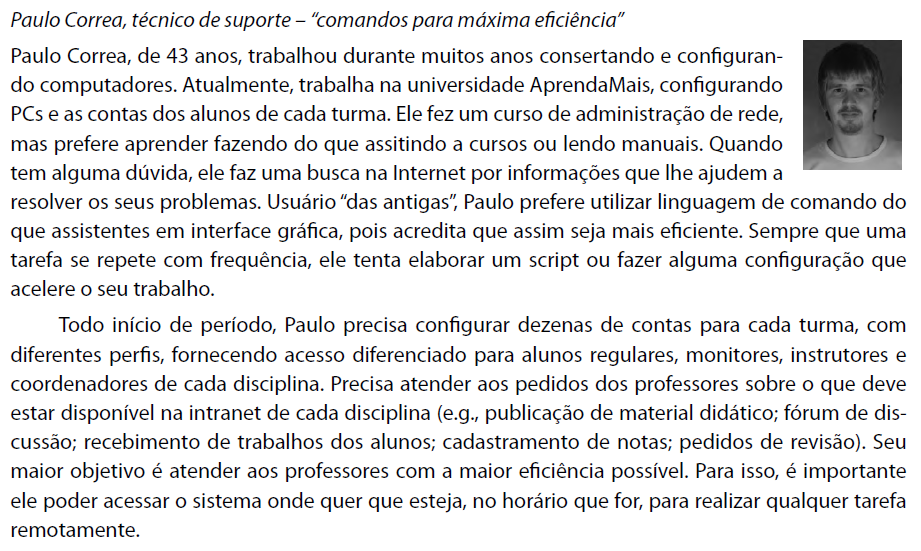
\includegraphics[keepaspectratio=true,scale=0.6]{figuras/metodologia/exemplo-persona.png}
	\legend{ Fonte: \citeonline{barbosa_silva} }
	\label{Fig:ex-persona.png}
\end{figure}

Elas são definidas a partir de dados de pesquisa de campo, ou seja, as personas refletem as características de pessoas reais. A pesquisa de campo envolve a coleta e uma pré-analise sobre o público-alvo, etapas as quais precedem a construção das personas \cite{usability2020}. 

Elas se caracterizam por atributos demográficos como sexo e faixa etária, atendem por um nome, além de conterem aspectos comportamentais, motivação e objetivos \cite[p. 81]{Vianna_2014}. Como é definido por \citeonline{Courage_Baxter_2005}, citado por \cite[p. 153-154]{BarbosaEtAl2021} uma persona possui as seguintes características: 

\begin{itemize}
    \item \textbf{identidade:} para dar mais realismo à persona, é importante que ela tenha um nome, idade, outros dados demográficos e uma foto;

    \item \textbf{status:} define o tipo das personas. Este atributo reflete a prioridade de uma persona classificando-a em primária, secundária, suplementar, cliente, servida ou anti-persona;

    \item \textbf{objetivos:} condição final a ser atingida, o alvo da persona. Os objetivos de uma persona não se restringem apenas ao produto, podendo ser por exemplo um objetivo pessoal, corporativo, técnico e prático;

    \item \textbf{habilidades:} atributo que reflete as especialidades, grau de escolaridade, capacidades e competências que não necessariamente devem estar relacionadas ao produto; 

    \item \textbf{tarefas:} aquilo que a persona executa, sendo elas básicas ou críticas. Elas ainda podem ser classificadas quanto a sua frequência, importância e duração;
    
    \item \textbf{relacionamentos:} quem a persona interage. Identificar com quem a persona se relaciona ajuda a mapear outras partes envolvidas ao projeto e que devem ser consideradas durante o processo de design;
    
    \item \textbf{requisitos:} aquilo que as personas precisam, suas necessidades; e
    
    \item \textbf{expectativas:} tanto o que a persona espera do funcionamento do produto, quanto aquilo que é gerado durante seu uso, na sua interação com o produto.
\end{itemize}

Como as personas partem de um processo de investigação das características dos usuários e descrição de seu perfil, a eficiência dessa ferramenta de design está atrelada ao quão próxima a persona se encontra de uma pessoa real e o quanto ela representa o seu público-alvo \cite[p. 154]{BarbosaEtAl2021}. 

Em um projeto podem haver um grupo de personas. Existem tipos distintos de personas, as quais tem um papel e prioridade sobre as outras \cite[p. 154]{BarbosaEtAl2021}. Na subseção a seguir este grupo de personas é melhor explorado.

\subsection{Elenco de Personas}

O grupo de personas de um projeto, também chamado de elenco de personas, conta com pelo menos três personas distintas como é definido por \citeonline{Courage_Baxter_2005} e \citeauthor{usability2020}, podendo ser de seis tipos, conforme foi descrito por \citeonline{cooper07}. São estes os tipos de personas:

\begin{itemize}
    \item Primária (\textit{Primary}): esta representa o principal alvo do design. Ela é que tem de ser satisfeita pela interface projetada;
    
    \item Secundária (\textit{Secundary}): esta é satisfeita com a interface projetada para a persona primária, porém a persona secundária necessita de adicionais específicas que podem ser acrescentadas ao design sem prejudicar aquilo que foi projetado para servir à persona primária;
    
    \item Suplementar (\textit{Supplemental}): ela é uma combinação das personas primárias e secundárias. Suas necessidades são completamente representadas por essa combinação de personas;
    
    \item Cliente (\textit{Customer}): esta persona busca atender às necessidades dos clientes, que não necessariamente são dos usuários finais do sistema;
    
    \item Servida (\textit{Served}): este tipo de persona é diferente do tipos de persona já discutidos. Ela não é um usuário do produto; contudo, eles são diretamente afetados pelo uso do produto; e
    
    \item Negativa (\textit{Negative}): chamada também de anti-persona, esta persona é usada para comunicar às partes interessadas e demais \textit{stakeholders} que existem tipos específicos de usuários para os quais o produto não foi projetado. 
\end{itemize}

O elenco de persona é caracterizado por conter ao menos uma persona por papel de usuário sendo que, dentre as personas definidas para cada papel, ao menos uma delas deve ser a persona primária. O ideal é que seja projetada uma interface distinta para cada persona primária \cite[p. 155]{BarbosaEtAl2021}. Por exemplo em um sistema escolar com dois papeis de usuário distintos, como alunos e professores, haveriam pelo menos duas personas primárias (uma representando os professores e outra os alunos), sendo que seria recomendado ser projetado duas interfaces distintas (novamente, uma para os professores e outra para os alunos).

\section{Jogos para Aprendizagem}
\label{sec:jogos-aprend}

Nesta seção é apresentada uma breve contextualização sobre jogos para aprendizagem, além dos elementos que envolvem a construção desse tipo de jogo e como eles se caracterizam. 
\subsection{Contextualização sobre Jogos para Aprendizagem}

A academia tem investigado o uso de abordagens inovadoras para auxiliar o processo de aprendizagem, instigando, atraindo e motivando o aluno no desenvolvimento de atividades pedagógicas \cite{battistella, brito, Sales2020}. Uma das abordagens exploradas é o uso de jogos. No geral, os jogos têm uma capacidade de atrair e motivar as pessoas e de gerar engajamento e dedicação na realização de tarefas \cite{Vianna_Vianna_Medina_Tanaka_Krug_2013}. 

O jogo sério é um tipo de jogo que vai além do entretenimento, o qual pode visar informar, treinar e ensinar. Esse tipo de jogo pode ser aplicado em diversas áreas, tais como saúde, publicidade, política e educação. Jogos sérios também incluem jogos para aprendizagem \cite{Becker_2021}.

No caso de ser aplicado na educação, os jogos para aprendizagem buscam tornar o processo de ensino-aprendizagem mais atrativo e proveitoso, desenvolvendo no estudante habilidades cognitivas através da prática e engajar os alunos nesse processo \cite{sommariva, queiroz, darin}. Dentro da educação existem várias áreas de conhecimento nas quais o jogos são aplicados no intuito de auxiliar o ensino e aprendizagem. Uma dessa áreas é a de Interação Humano-Computador \cite{Sales2020, Sales2020UsoTDS}. 

Jogos para aprendizagem é um tipo de abordagem que vem se tornando cada vez mais popular na educação em computação, pois podem aumentar a eficácia e o engajamento da aprendizagem \cite{battistella, brito, sales_climaco2016, queiroz}. Na subseção a seguir são exploradas as características deste tipo de jogo e o que envolve seu desenvolvimento.

\subsection{Desenvolvimento e Características de Jogos Digitais para Aprendizagem}

Um processo sólido para se desenvolver um jogo que parte da concepção de uma ideia e objetiva chegar em um resultado que promova uma experiência satisfatória ao jogador, é a chave para se construir um \textit{game} \cite[p. 10-11]{Fullerton_2008}.  Segundo \citeonline[p. 10-11]{Fullerton_2008} esta é uma abordagem centrada no jogador, na qual o princípio é envolver o jogador no processo de design do início ao fim, ou seja, manter continuamente a experiência do jogador como o alvo a ser atingido, além de testar a jogabilidade com os jogadores-alvo durante as etapas de desenvolvimento.

O \textit{Playcentric Design Process} (PDP) é um método de desenvolvimento de jogos, que segue esse princípio de envolver o jogador. Nele, o jogador é inserido no processo logo cedo ao serem definidas as metas de experiência do jogador \cite{Fullerton_2008}.

O PDP se baseia num ciclo iterativo, no qual continuamente é prototipado, testado e validado o que foi concebido para o jogo, sempre tendo em vista as metas de experiência \cite[p. 10-11]{Fullerton_2008}. Este método acompanha a visão de IHC que preocupa-se com certos critérios de qualidade da interação entre seres humanos e sistemas digitais \cite[p. 8-10]{BarbosaEtAl2021}.

\citeonline{BarbosaEtAl2021} apontam que ``os critérios de qualidade de uso enfatizam certas características da interação e da interface que as tornam adequadas aos efeitos esperados do uso do sistema". São critérios de qualidade, a usabilidade e a experiência do usuário (UX).

\citeonline{Petri_Wangenheim_2019} abordam em seus estudos a questão da qualidade em jogos educacionais e trazem como produto de suas pesquisas um modelo denominado Model for the Evaluation of Educational Games (MEEGA+). Este é um instrumento de avaliação da qualidade de jogos no ensino de informática que contempla fatores de usabilidade e experiência do jogador (Anexo \ref{an:meega}).

Os fatores de qualidade do MEEGA+ ainda são decompostos em dimensões. Estas dimensões descrevem as características dos jogos educacionais que impactam na qualidade deles \cite{Petri_Wangenheim_2019}.

Outro estudo similar que aborda a caracterização de jogos para aprendizagem é o de \citeonline{deSales_SousaeSilva_2020}. Neste trabalho são contemplados os requisitos de qualidade, a experiência do jogador, além de outras características gerais de jogos sérios no processo e ensino e aprendizagem de IHC. 

Estas características de jogos, tal como suas respectivas relevâncias, foram observadas no estudo de \citeonline{silva_sales_mendes2021} como aspectos de qualidade. Estes aspectos refletem critérios, princípios de \textit{design} \cite{nielsen1994, ISO9126-1, BarbosaEtAl2021}, metas de usabilidade e aspectos de experiência desejáveis do usuário \cite{Preece_Rogers_Sharp_2005} identificados na Engenharia de Software (ES) e em IHC.

Estes aspectos de qualidade são para os designers e desenvolvedores, os insumos fundamentais do processo de desenvolvimento para esse tipo de \textit{software} \cite{silva_sales_mendes2021}. Neste processo, a Engenharia de Software aborda, a etapa de entendimento dos elementos que envolvem o tema do projeto de um software é denominada de concepção do projeto \cite[p. 127]{Pressman_2000}.

Após a concepção, os aspectos de qualidade ganham forma, sendo especificamente modelados para determinado projeto \cite[p. 151]{BarbosaEtAl2021}. A exemplo de modelagem existem as personas, que no caso incorporam estes aspectos de qualidade \cite[p. 154]{BarbosaEtAl2021}.

No desenvolvimento de um software estes aspectos de qualidade podem ser traduzidos para requisitos não funcionais \cite{swebok2014} e para as metas de experiência do usuário, as quais fazem parte de atividades na engenharia de software, como a prototipação, inspeção, validação e testes \cite{Pressman_2000}.

\section{Trabalhos Correlatos}
\label{sec:trab_cor}

Nesta seção são apresentados trabalhos que têm algumas similaridades com o presente estudo. Estes envolvem a construção de personas para o desenvolvimento de um jogo, outro para um jogo na educação e ainda um que trata do uso de \textit{survey} para se elaborar personas.

No trabalho de \citeonline{canossa-2009} personas são desenvolvidas com o intuito de solucionar o desafio de integrar o usuário ao design de entretenimento interativo (jogos de computador). Este trabalho utiliza a estrutura introduzida por \citeonline{cooper99}.

As personas desenvolvidas neste estudo são conhecidas também como \textit{play-personas}. Com base num estudo de caso da pesquisa de \citeonline{canossa-2009}, as \textit{play-personas} se mostraram como modelos de hipótese preliminar de comportamento no jogo e uma ferramenta para categorizar e analisar variáveis de métricas de jogo vinculadas ao personagem.

A estrutura adotada para a \textit{play-persona} agrega os dados coletados, vinculando-os aos aspectos de jogos. Estes aspectos vão além de meras recompensas e punições, mas sim, envolvem desafios e habilidades referentes a um público indistinto em geral \cite{canossa-2009}.

Outro trabalho que liga jogos e personas, é o estudo de \citeonline{salminen-2020}. Este estudo conta com a aplicação de uma pesquisa com \textit{survey} para coleta de dados que serviram de insumo par a construção das personas. 

Assim foram geradas personas de forma automática, a partir da base de dados de preferências de jogos e demais características dos usuários, coletadas via formulário digital \cite{salminen-2020}.

As personas resultantes podem ser aplicadas direcionando os jogadores, com publicidade em mídia social, para jogos de sua preferência. Além disso elas também podem ser usadas para compreender a variação demográfica entre vários padrões de preferência de jogo \cite{salminen-2020}.

Por último, mas não menos importante o trabalho de \citeonline{Salomao_2015} usou da técnica de personas para o desenvolvimento do protótipo de um jogo digital e na continuação deste trabalho \cite{Salomao_2016}, o próprio jogo foi desenvolvido e então as personas avaliadas para se ter o entendimento se de fato elas refletiram os jogadores.

Neste trabalho \cite{Salomao_2015} os dados das personas foram coletados e analisados a partir de 30 entrevistas com potenciais usuários (estudantes internacionais que residiam no Brasil e Portugal com interesse em aprender português como língua estrangeira). Estes tiveram elementos repetidos como itens mais citados na análise de conteúdo pelo grupo de alunos (entrevistas de falantes de espanhol morando no México) que avaliaram a versão final do jogo. Essa evidência indica a robustez da Persona que norteou o design do jogo \cite{Salomao_2016}.

Estes trabalhos apresentam diferentes abordagens do uso de personas no processo de design de jogos. \citeonline{canossa-2009} apresenta a perspectiva centrada no usuário envolvendo aspectos de jogos e experiências do jogador em sua análise. Já \citeonline{salminen-2020} envolve o uso do \textit{survey} para coleta dos dados utilizados na modelagem das personas. E \citeonline{Salomao_2015, Salomao_2016} apresentam o uso e a avaliação das personas usadas no projeto de um jogo na educação.

No presente trabalho, tanto a visão centrada no usuário, envolvendo aspectos de qualidade de jogos, quanto o uso do \textit{survey} como procedimento para coleta dos dados para a construção das personas e o objetivo de se desenvolver um jogo para aprendizagem, são aqui abordados. Dito isto, no Capítulo \ref{chap:Metodo} estão apresentadas as metodologias adotadas neste trabalho.